\documentclass[12pt,letterpaper]{article}
\usepackage{graphicx,textcomp}
\usepackage{natbib}
\usepackage{setspace}
\usepackage{fullpage}
\usepackage{color}
\usepackage[reqno]{amsmath}
\usepackage{amsthm}
\usepackage{fancyvrb}
\usepackage{amssymb,enumerate}
\usepackage[all]{xy}
\usepackage{endnotes}
\usepackage{lscape}
\newtheorem{com}{Comment}
\usepackage{float}
\usepackage{hyperref}
\newtheorem{lem} {Lemma}
\newtheorem{prop}{Proposition}
\newtheorem{thm}{Theorem}
\newtheorem{defn}{Definition}
\newtheorem{cor}{Corollary}
\newtheorem{obs}{Observation}
\usepackage[compact]{titlesec}
\usepackage{dcolumn}
\usepackage{tikz}
\usetikzlibrary{arrows}
\usepackage{multirow}
\usepackage{xcolor}
\newcolumntype{.}{D{.}{.}{-1}}
\newcolumntype{d}[1]{D{.}{.}{#1}}
\definecolor{light-gray}{gray}{0.65}
\usepackage{url}
\usepackage{listings}
\usepackage{color}
\usepackage{subcaption}

\definecolor{codegreen}{rgb}{0,0.6,0}
\definecolor{codegray}{rgb}{0.5,0.5,0.5}
\definecolor{codepurple}{rgb}{0.58,0,0.82}
\definecolor{backcolour}{rgb}{0.95,0.95,0.92}

\lstdefinestyle{mystyle}{
	backgroundcolor=\color{backcolour},   
	commentstyle=\color{codegreen},
	keywordstyle=\color{magenta},
	numberstyle=\tiny\color{codegray},
	stringstyle=\color{codepurple},
	basicstyle=\footnotesize,
	breakatwhitespace=false,         
	breaklines=true,                 
	captionpos=b,                    
	keepspaces=true,                 
	numbers=left,                    
	numbersep=5pt,                  
	showspaces=false,                
	showstringspaces=false,
	showtabs=false,                  
	tabsize=2
}
\lstset{style=mystyle}
\newcommand{\Sref}[1]{Section~\ref{#1}}
\newtheorem{hyp}{Hypothesis}

\title{Disproportionate policy dynamics in crisis and uncertainty: an international comparative analysis of policy responses to COVID-19\footnote{Shafi, S. and Mallinson, D. J. (2022) "Replication Data for: Disproportionate Policy Dynamics in Crisis and Uncertainty: An International Comparative Analysis of Policy Responses to COVID-19", Harvard Dataverse, V1. Available at: https://doi.org/10.7910/DVN/MABPEC (Accessed 15 April 2024)}}
\date{Submitted: 15 April 2024}
\author{Replication Project}


\begin{document}
	\maketitle
	\section*{Can we assess the impacts of policy responses on pandemic outcomes?}
	
	\vspace{.25cm}
	
	\noindent Shafi and Mallinson (2023)\footnote{Shafi, S. and Mallinson, D. J. (2023) "Disproportionate Policy Dynamics in Crisis and Uncertainty: An International Comparative Analysis of Policy Responses to COVID-19", Policy Studies, 44 (1), pp. 09-111. Available at: https://doi.org/10.1080/01442872.2022.2053093 (Accessed 15 April 2024)} employ \textbf{pooled panel linear regression} using \textbf{weekly time series data for 160 countries from 27 Jan to 27 Dec 2020} to explore the dynamics between state responses during the first year of the COVID-19 pandemic and reported cases of and deaths from the virus. The paper aims to fill existing knowledge gaps in the literature around the \textit{dynamics} and the \textit{outcomes} of different policy approaches across countries.
	
	\vspace{.25cm}

%	\noindent The paper highlights limitations in existing theoretical frameworks for defining and evaluating disproportionate policy responses (over- and under-) during crises such as the COVID-19 pandemic; especially regarding decision-making under high-threat and high-uncertainty conditions. Further, the paper acknowledges temporal aspects of both pro-active and reactive policy change as crises and politics progress and transform as new information and conditions emerge.
%	\vspace{.25cm}
		
	\noindent The authors' findings indicate that increased income supports and debt relief are associated with fewer COVID-19 deaths up to four weeks, and potentially beyond, while "broad policy interventions" across all economic, health, and social dimensions are associated with short-term reductions in the weekly rate of deaths.
	
	\vspace{.25cm}
		
	\noindent This paper is an excellent case study for replication as it provides largely thorough and readable data and code for reproducing results in R, alongside documentation for the secondary data used. However, the published paper and provided code include errors of a minor and serious nature, which are highlighted in a dedicated section of this report. Also note that the numbering of figures in this paper does not consistently match those in the original report - the title will remain the same for easier reference between the two documents.
	
	\vspace{.25cm}
	
	\noindent I chose this specific paper for replication as it is thematically relevant to 2024's international policy context, and comparative policy analysis more broadly, as well demonstrates advanced methodology which is relevant to my own interests in comparative policy analysis and data-informed policy research.
	
	\vspace{.25cm}

	\section*{Errors in the Paper and Data}
	
	\vspace{.25cm}
	
	\noindent There is a numbering typo error on line 400 which I corrected. Further, the code for Figures 4 and 5 is absent, most likely an accidental exclusion. As they are not essential plots for the overall discussion or for replication purposes, I did not attempt to reproduce these plots.
	
	\vspace{.25cm}
	
	\noindent In the paper and replication code, the first figure erroneously plots the Stringency Index for France in all four graphs, where each plot should show the country's progression across the Containment Health, Government Response, and Economic Support indices respectively. While this does not impact the overall findings of the paper, I show the published and the corrected plots side-by-side in Figure 1 below. Additionally, the original plotting of the results for the GRI models includes an error in the x-axis of the fourth subplot for "New Weekly Deaths". This is also a minor graphical error and I do not correct it when comparing the results from the original paper and the updated models.
	
	\vspace{.25cm}
	
	\noindent More seriously, the replicated results of the Hausman Tests, which assess if the fixed-effect models are more appropriate than the random-effect models, are contrary to what the paper reports - regarding the GRI model presented by the authors for discussion, one result is consistent, while the remaining three are not.
	
	\vspace{.25cm}
	
	\noindent Further, within the replication code, these tests are only conducted for the \texttt{Government Response Index}, and not for the \texttt{Stringency}, \texttt{Economic Support} nor \texttt{Containment Health} indices - this is despite the authors explicitly reporting that these tests were conducted and returned overall conclusive results supporting their argument "that a fixed effects model was the most efficient, and thus preferred,  model ($p < 0.05$)" (Shafi and Mallinson, 2023, p. 98). Therefore, alongside the contradictory results from what is included in the replication code, the exclusion of these other tests' code is problematic.
	
	\vspace{.25cm}
	
	\noindent However, due to resource constraints, I do not perform these tests on the original models and instead follow the remaining steps of the authors' analysis in order to demonstrate the impacts of my "twist". Note I have included the raw code below as the \texttt{stargazer} package in R does not support Heusman Test tables as of the time of writing.
	
	\lstinputlisting[language=R, firstline=1276, lastline=1282]{COVID Policy Reproduction Code 2022-02-21.R}
	
	\vspace{.25cm}

\newpage
	\section*{What is the data used?}
	\vspace{.25cm}
	\noindent For data on COVID-19 policy responses, this paper uses four indices from the \textit{Oxford COVID-19 Government Response Tracker} (OxCGRT)\footnote{Thomas Hale, Noam Angrist, Rafael Goldszmidt, Beatriz Kira, Anna Petherick, Toby Phillips, Samuel Webster, Emily Cameron-Blake, Laura Hallas, Saptarshi Majumdar, and Helen Tatlow (2021) “A global panel database of pandemic policies (Oxford COVID-19 Government Response Tracker).” Nature Human Behaviour. Available at: https://doi.org/10.1038/s41562-021-01079-8 or https://github.com/OxCGRT/covid-policy-tracker}, with minor modifications for the purposes of the study:
	\begin{itemize}
		\item Stringency index
		\item Government response index
		\item Economic support index
		\item Containment health index
	\end{itemize}
	
	\noindent These are 'nested' indices, meaning each index uses a subset of the same 23 indicators of government policy responses to the COVID-19 pandemic. As illustrated in Figure 1 (see in the next section), this leads to similar trends across all four indices internationally.
	\vspace{.25cm}
	
	\noindent The paper also draws from \textit{World Development Indicators} (WDI) datasets from the World Bank\footnote{World Bank (2020) "World Development Indicators", 1 July, World Bank. Available at: https://datacatalog.worldbank.org/dataset/world-development-indicators (Accessed 7 August 2020)} as well as the World Health Organisation\footnote{World Health Organization (2020) "WHO Coronavirus Disease (COVID-19) Dashboard", World Health Organzation. Available at: https://covid19.who.int/ (Accessed 11 July 2020)} and the World Meters platform \footnote{World Meters (2020) "Coronavirus Cases". Available at: https://www.worldometers.info/coronavirus/coronavirus-cases/ (Accessed 7 October 2020)} for control variables, including total population, total population aged 65 and over,population density, and GDP per capita.
	\vspace{.25cm}
	
	\noindent Once loaded, the authors cleaned and modified/transformed the data for analysis, for example, normalising population measures for better comparability across countries of different sizes, and log transformations on measures of fiscal and emergency investment measures as their distributions skewed to the right. All modifications are specified included within the replication code.

	\section*{What are the research questions?}
	\vspace{.25cm}
	
	\noindent While the authors acknowledge the preliminary nature of the analysis, the empirical validity of the paper's results remains questionable - in addition to the aforementioned inconsistent results supporting the methodology, the manuscript does not explicitly state nor test hypotheses drawn from the three stated research questions - rather, the paper uses descriptive analysis and theoretical arguments to connect analyses and results to its three research questions. Below I highlight the key features of the paper's analysis:
	
	\begin{enumerate}
		\item Have countries pursued consistently disproportionate policy responses throughout the pandemic? Is there evidence that countries have pursued intentional or nonintentional disproportionate policymaking?
		
		\begin{itemize}
			\item Figure 1 shows significant variation in the policy responses over the first year of the COVID-19 pandemic, highlighting France and the US as examples.
			%\item Figures 4 and 5 illustrate how some countries 'under-' and 'over'-reacted across time, with different countries at different time points, where changes in policy response levels appear to correlate with texttt{New Daily Cases}. As the replication code does not include these figures, I do not attempt to recreate them and have copied the plots directly from the paper.
			\item Note that the authors take correlation between government response and daily cases as indicative of \textit{intentionality} (or non-) and \textit{pro-activity} (or reactivity) of national-level policymaking, though neither theoretical evidence nor statistical analysis is provided to substantiate this causal claim.
			
			\begin{figure}[htp]
				\centering
				\begin{subfigure}[b]{0.8\textwidth}
					\centering
					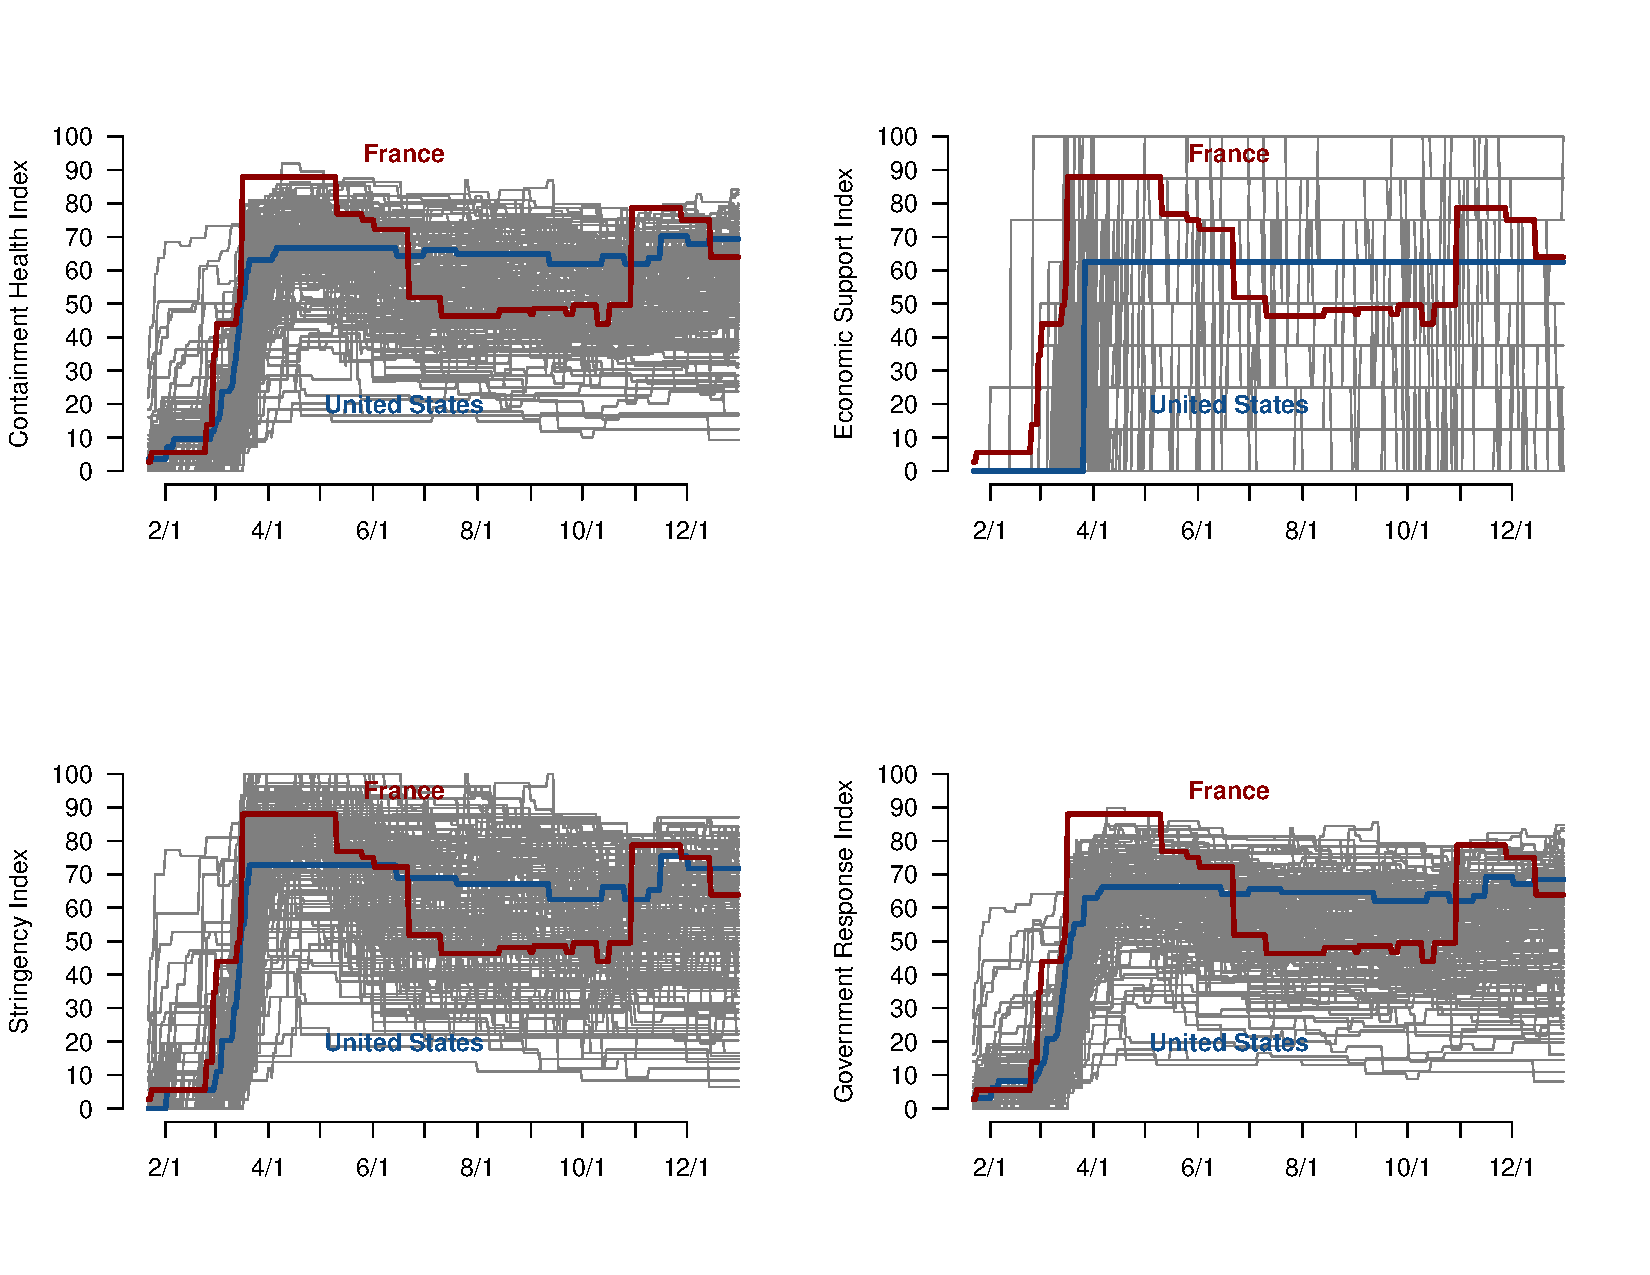
\includegraphics[width=\textwidth]{figure1.pdf}
					\caption{Published Graphic}
					\label{fig:figure1}
				\end{subfigure}
				\hspace{0.05\textwidth} % Adjust the horizontal space between subfigures
				\begin{subfigure}[b]{0.8\textwidth}
					\centering
					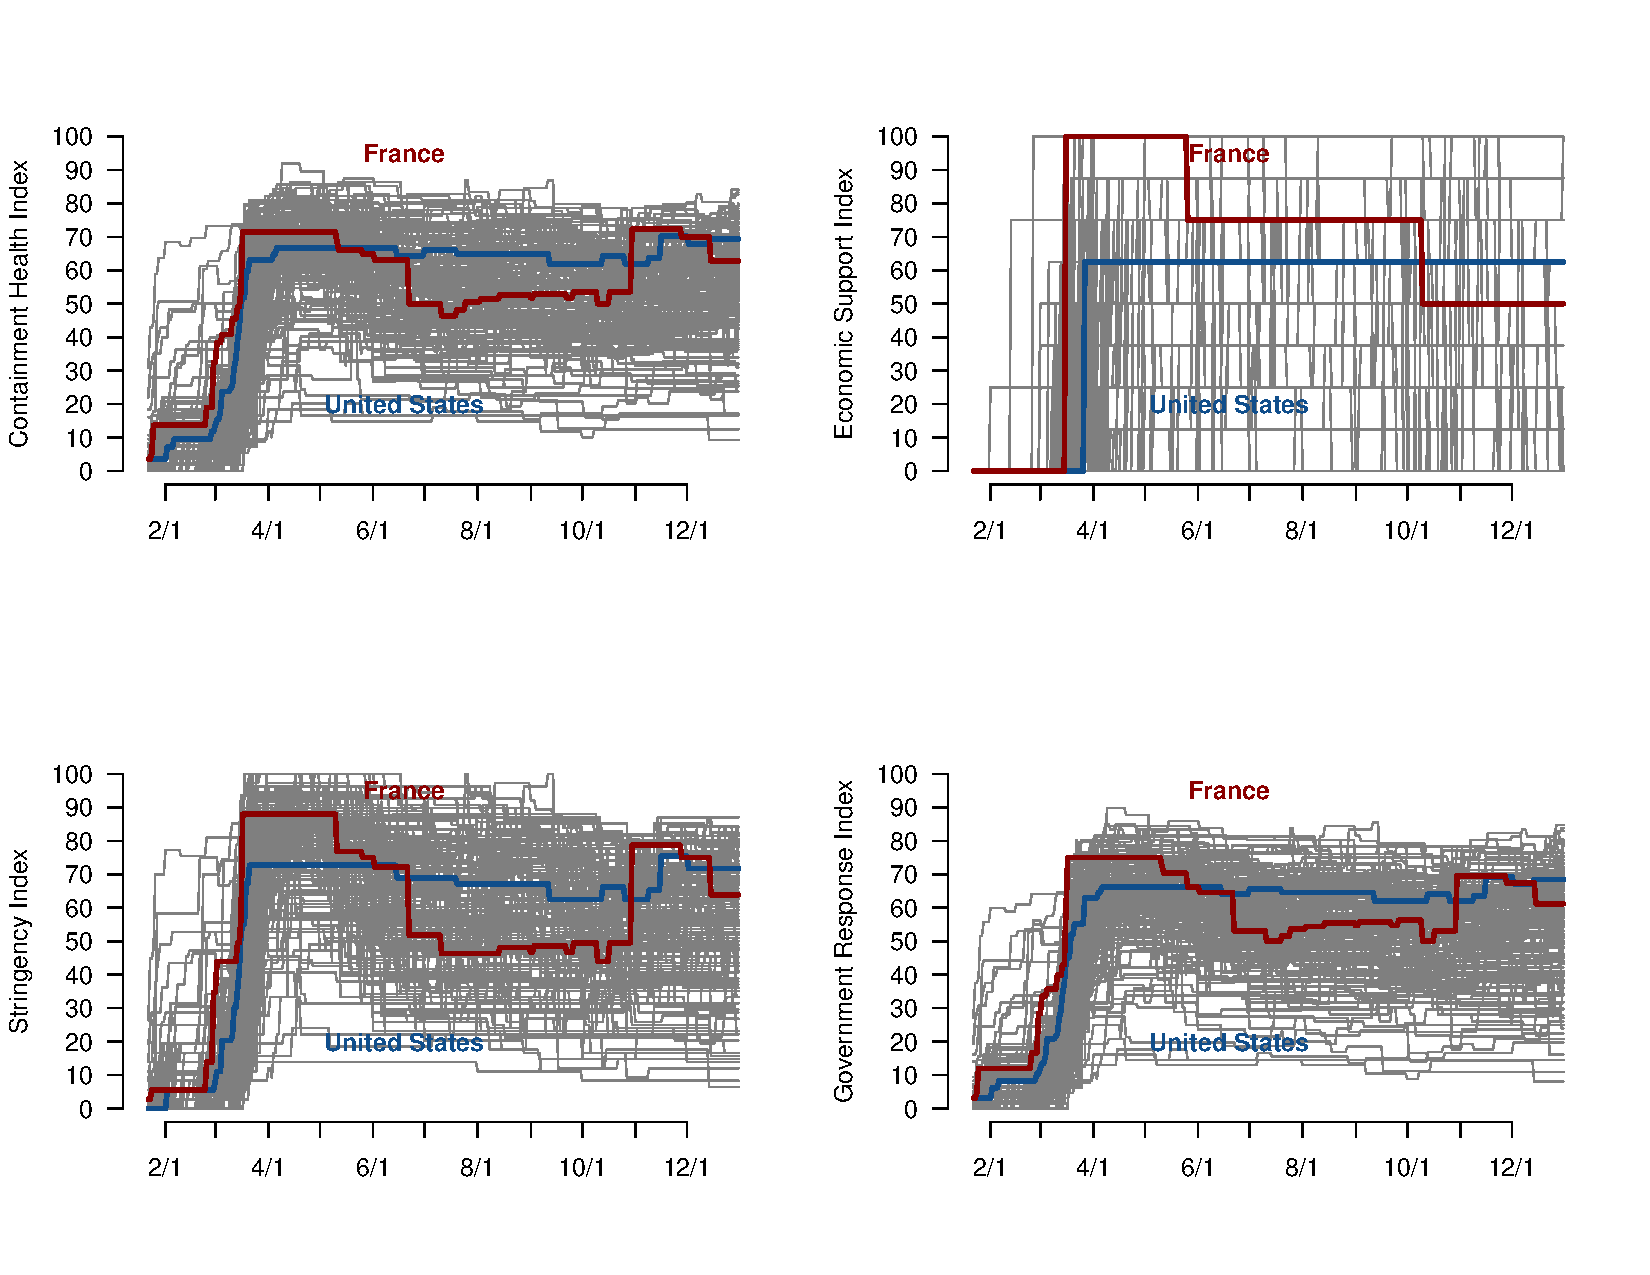
\includegraphics[width=\textwidth]{figure1_corrected.pdf}
					\caption{Corrected Graphic}
					\label{fig:figure1_corrected}
				\end{subfigure}
				\caption{COVID-19 Policy Response Indices from January to December 2020}
				\label{fig:figure1_both}
			\end{figure}
			
%			\begin{figure}[h!]
%				\centering
%				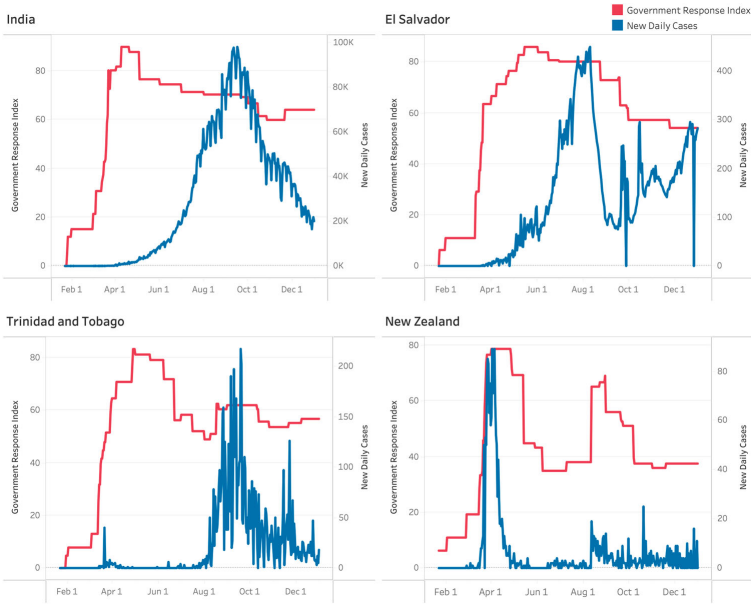
\includegraphics[width=0.8\textwidth]{figure4_screenshot.png}
%				\caption{Policy Over-Reactions at the Time of Maximum Response [Screenshot from paper]}
%				\label{fig:figure4}
%			\end{figure}
%			\begin{figure}[h!]
%				\centering
%				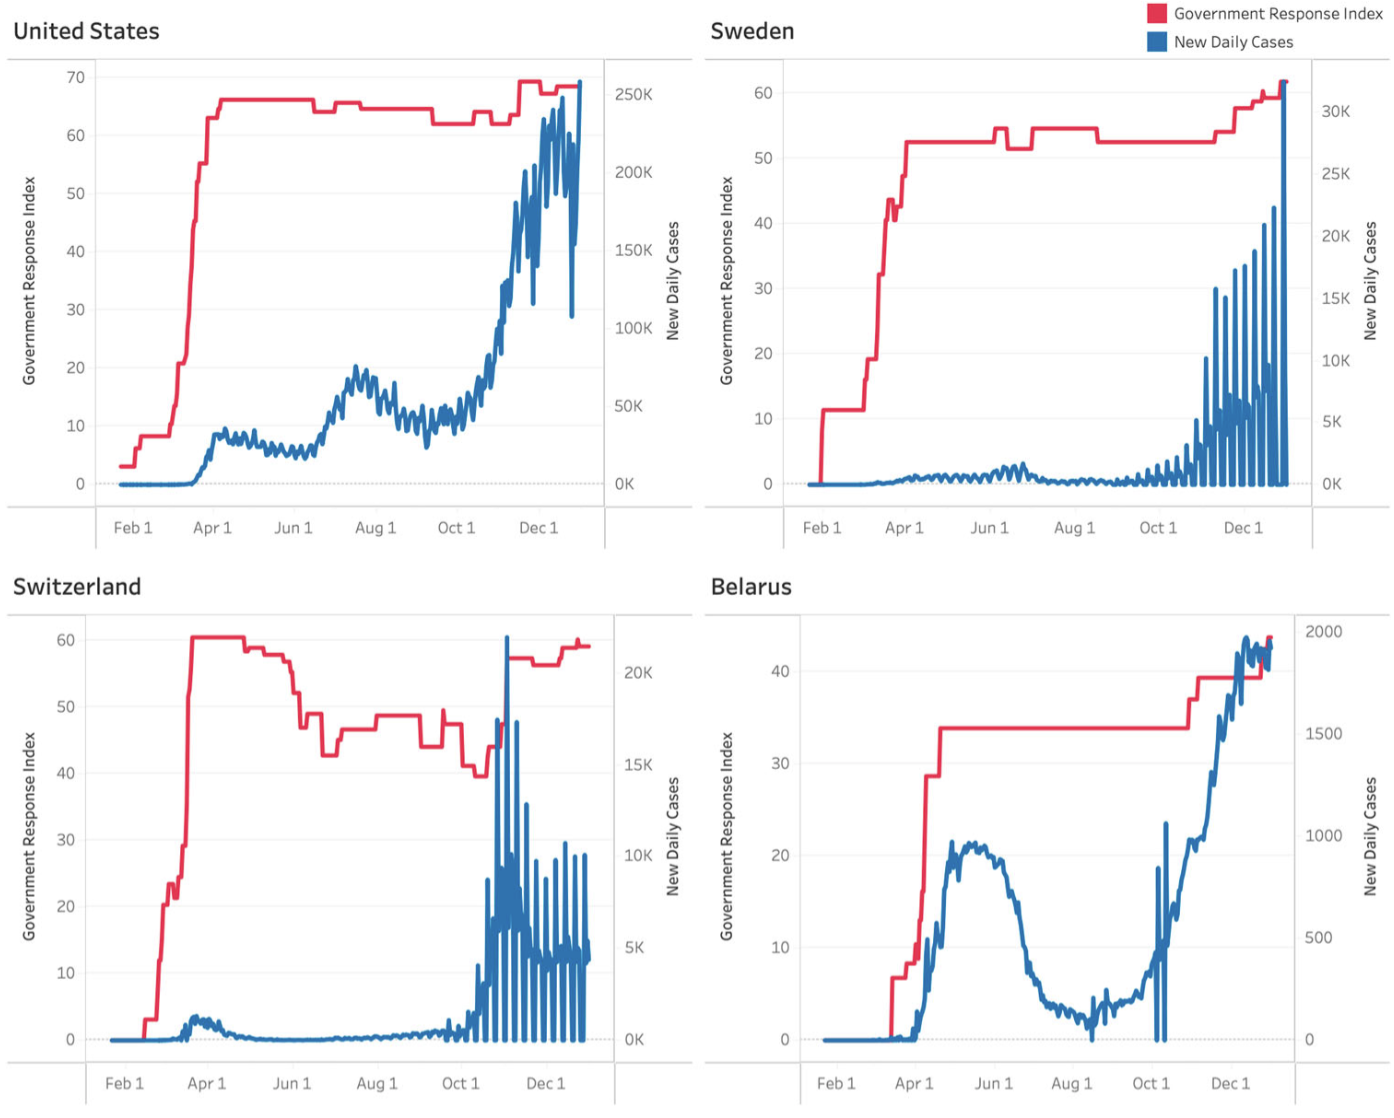
\includegraphics[width=0.8\textwidth]{figure5_screenshot.png}
%				\caption{Policy Under-Reactions at the Time of Maximum Response
%					[Screenshot from paper]}
%				\label{fig:figure5}
%			\end{figure}
			
		\end{itemize}
		
		\item Are countries with more stringent policy responses more effective in managing the public health crisis than countries with less stringent policy responses?
		
		\begin{itemize}
			\item Figure 2 plots the risk-response ratios for each countries with a smoothed line of best fit. Results are inconclusive as evidence for stringency correlating with COVID-19 outcomes, and the authors point to potential sources of error in
			
			\begin{enumerate}
				\item the relative nature of the risk-response ratio classification process (as an absolute scale may capture the true magnitudes of variation and disparity between policy responses), and
				\item the model's exclusion of contextual factors such as socio-cultural, political and economic dimensions which uniquely impact individual national contexts.
			\end{enumerate}
			
			\item The latter point is especially pertinent, as the power dynamics and pressures from social and political contexts are highly influential on state-level decision-making. While this is a provisional study, neglecting national socio-political contexts undermines any findings from a paper oriented towards exploring the dynamics and outcomes of policymaking in crisis contexts.
		
			\begin{figure}[ht]
				\centering
				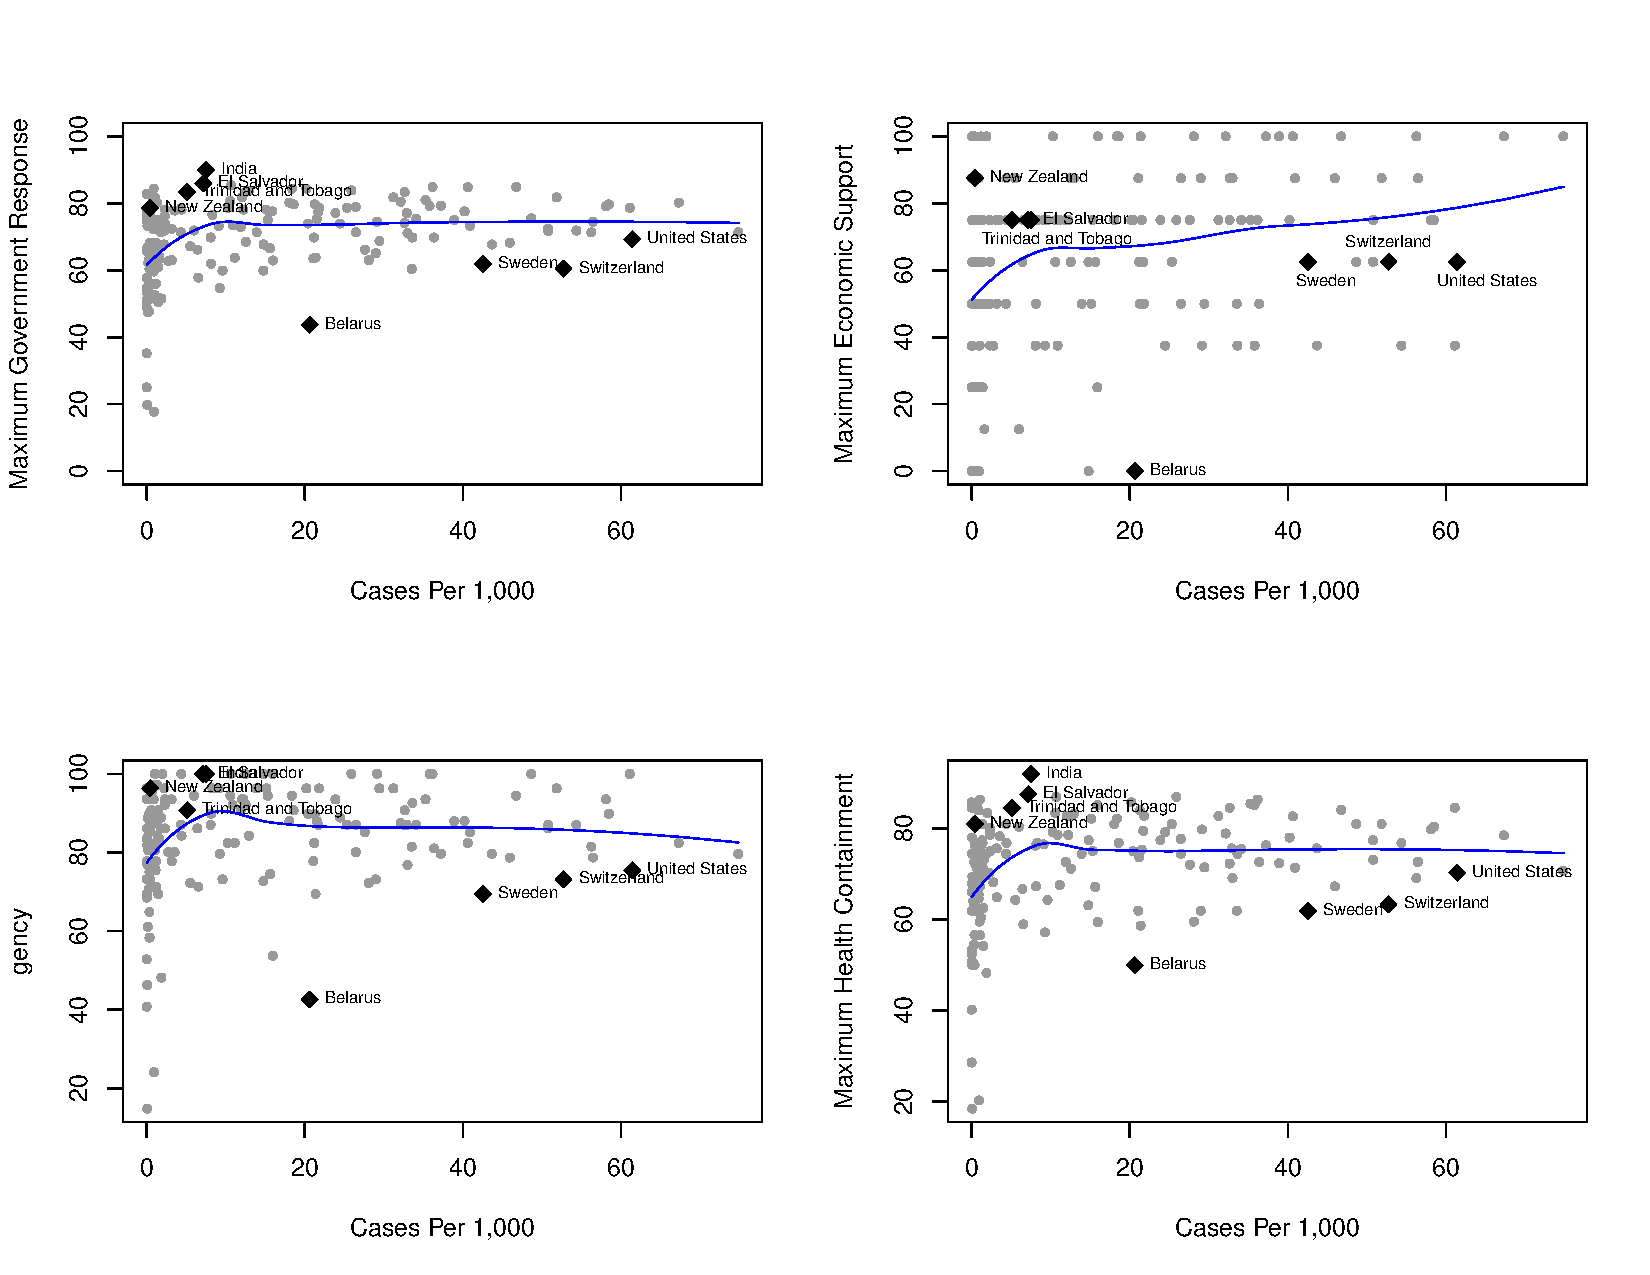
\includegraphics[width=0.7\textwidth]{figure3.pdf}
				\caption{Policy Over- and Under-Response to COVID-19 [Replicated]}
				\label{fig:figure3}
			\end{figure}
		\end{itemize}
		
		\item Which types of policies — containment, economic, or health — have proven most
		effective in managing the public health crisis?
		
		\begin{itemize}
			\item The authors highlight evidence that "economic support policies have proven most effective in managing the public health crisis", naming income support and debt/contract relief as associated with a fall in the rate of deaths for up to four weeks, while "broad" interventions for containment, health, and economic supports reflect reductions in the same for a week from their implementation, but not beyond this time frame (Shafi and Mallinson, 2023, p. 107-8).
			
			\item Figure 3 illustrates that the largest log-odds coefficient for \texttt{Economic Support Index} on \texttt{New Weekly Deaths} lags by 3 weeks, and still holds up to 4 weeks. Results for most other measures are less notable.
			
			\item While the aggregated global-level results inform the authors' insights, the use of national-level indicators to identify singular policy responses as generally the 'best' across across the international community is problematic, given the wide variation in social and political contexts, as well the influence of unique national features on policy responses and outcomes, such as the nature of employment and in which sectors, and the variation in actual implementation of particular policy responses. The authors acknowledge that precisely these dimensions are not captured within this analysis, which further undermines any insights which may be drawn from these results.
			
			\begin{figure}[!h]
				\centering
				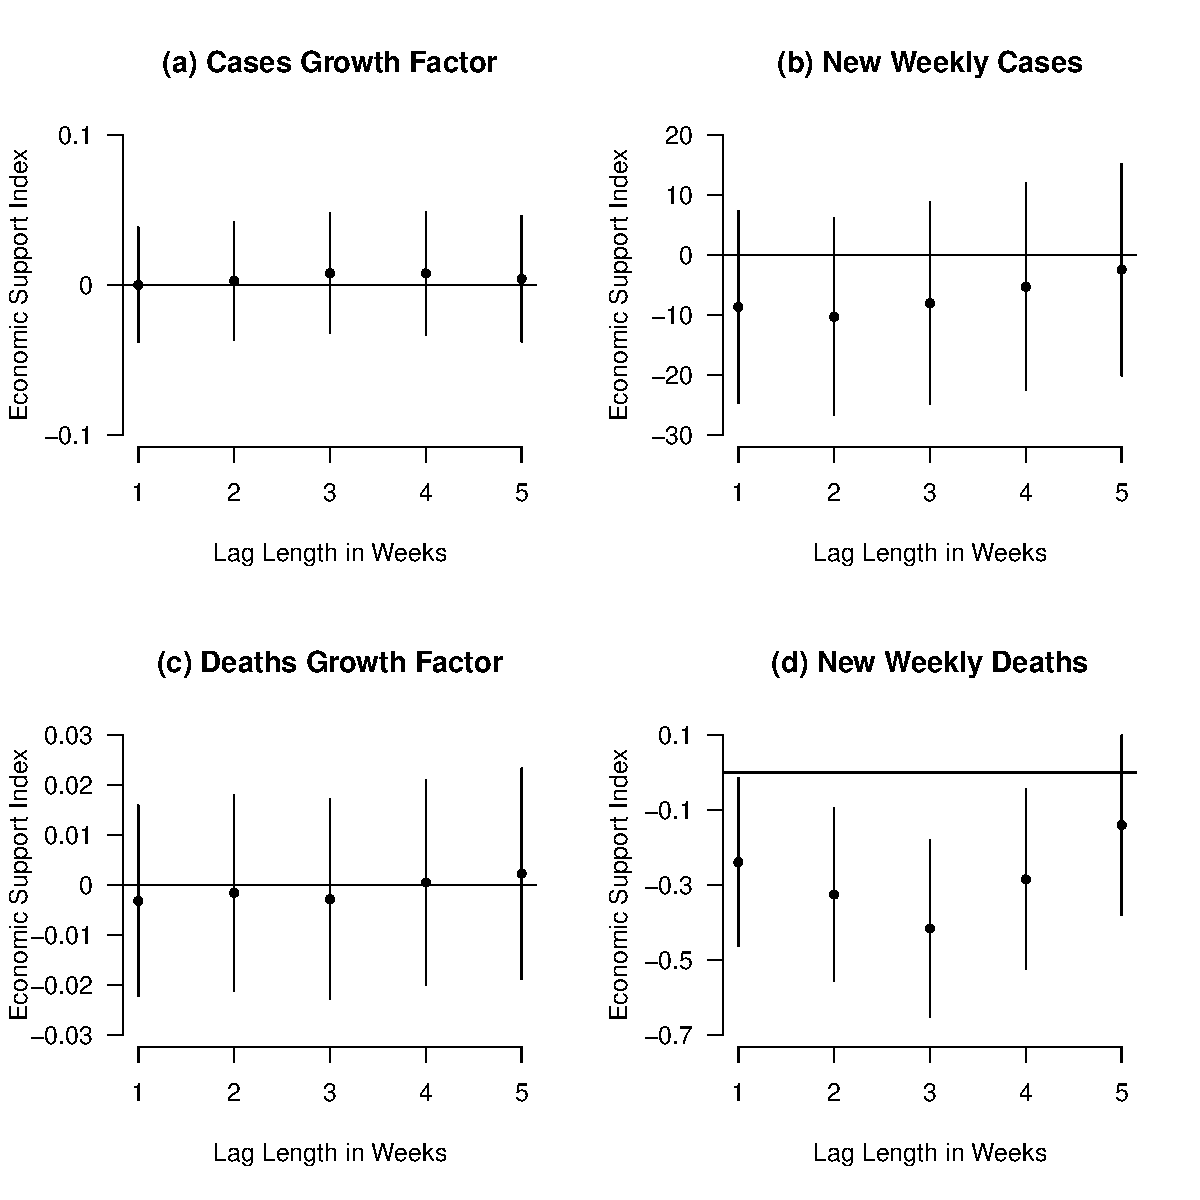
\includegraphics[width=0.7\textwidth]{esi.pdf}
				\caption{Economic Support Index Coefficients across Four COVID-19 Outcomes, Lagged 1–5 Weeks [Replicated]}
				\label{fig:esi}
			\end{figure}
		\end{itemize}
	\end{enumerate}
	
	\section*{What is my 'twist'?}
	
	\vspace{.25cm}	
	
	\noindent A key dimension to the paper's analysis is the nature of Over- and Under-Response to COVID-19, with countries above / to the left of the smoothed regression line classified the former, and those below / to the right as the latter. However, the paper does not directly compare these two groupings of country responses. I argue there are systematic differences between countries which consistently respond 'above' the average rate to those 'below'.
	
	\vspace{.25cm}	
	
	\noindent By repeating analyses with subsets of "Over-Responders" and "Under-Responders" (defined according to relative position to the smoothed regression line, as specified by the authors), I expect to highlight these systematic differences, which later analyses including socio-political dimensions may capture with more precision:
	
	\lstinputlisting[language=R, firstline=1305, lastline=1324]{COVID Policy Reproduction Code 2022-02-21.R}

	\lstinputlisting[language=R, firstline=1327, lastline=1334]{COVID Policy Reproduction Code 2022-02-21.R}
	
%	\vspace{.25cm}
	\noindent Next, I reproduce the original paper's first figure (see Figure 4) to illustrate how 
	\begin{itemize}
		\item[a)] countries can be visually grouped by their Over- or Under-responsiveness, though the boundaries between these clusters are not clearly distinguishable, and
		\item[b)] the Averages across the two groups diverge from late March/early-April 2020, perhaps by the greatest magnitude across the Economic Support Index (which is especially notable as economic supports are highlighted by the authors as the most significant measures associated with reduced COVID-19 deaths across all countries).
	\end{itemize}
	
	\vspace{.25cm}
	
	\noindent Note, I use the \texttt{ggplot2} package due to challenges with representing additional graphic features effectively using Base R's capabilities (see lines \texttt{1336 to 1495}, or print the code directly in this paper by modifying the comment below in the given LaTeX file).
	
	%\lstinputlisting[language=R, firstline=1336, lastline=1496]{COVID Policy Reproduction Code 2022-02-21.R}
	
	\begin{figure}[h]
		\centering
		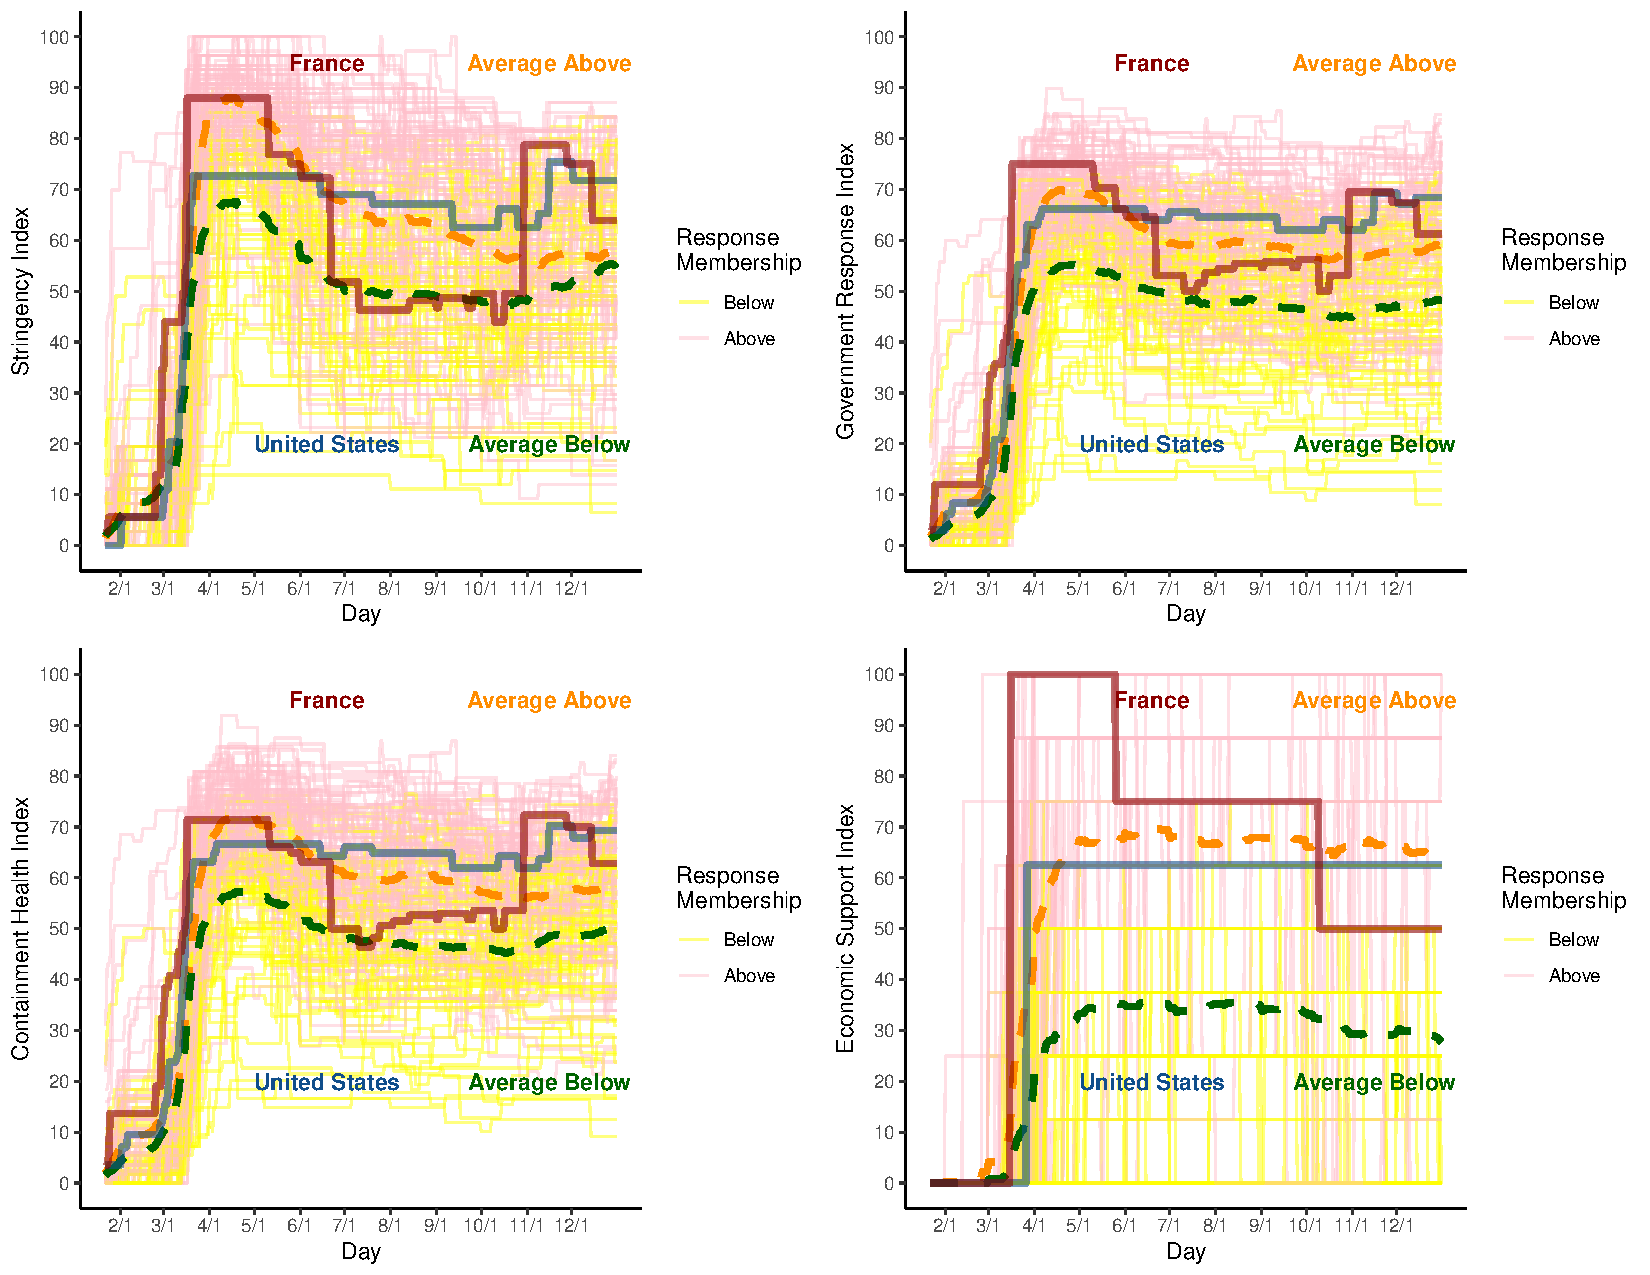
\includegraphics[width=1.05\textwidth]{all_plots1.pdf}
		\caption{COVID-19 Policy Response Indices from January to December 2020 (Updated)}
		\label{fig:figure1_new}
	\end{figure}
	
	
	\section*{Updated Results}
	
	\vspace{.25cm}	
	
	\noindent In line with the author's analysis, I perform \textbf{Hausman Tests} on the updated Fixed-Effect models based on subsets of "Over-Response" and of "Under-Response" classes for each index, with results indicated in Tables 1-3. Notably, the updated fixed-effects GRI models for Over-Response countries are "preferred" for three out of four outcomes, over one of four in the corresponding original models. This is the terminology used by the authors, and so I adopt this for comparing the original and updated approach.
	
	\begin{table}[ht]
		\centering
		\caption{Hausman Test Results: Government Response Index (Original)}
		\label{tab:hausman_test1}
		\begin{tabular}{lccc}
			\hline
			\textbf{Outcome} & \textbf{Chi-squared} & \textbf{Degrees of Freedom (df)} & \textbf{p-value} \\
			\hline
			Cases Growth Factor & 2.1981 & 4 & 0.6994 \\
			New Weekly Cases & 0.69163 & 4 & 0.9524 \\
			Deaths Growth Factor & 4.8157 & 4 & 0.3067 \\
			New Weekly Deaths & 84.324 & 4 & $< 2.2 \times 10^{-16}$ \\
			\hline
		\end{tabular}
		\begin{flushleft}
			\emph{Note:} The null hypothesis is that the models are consistent. The alternative hypothesis is that one model is inconsistent.
		\end{flushleft}
	\end{table}
	
	\begin{table}[ht]
		\centering
		\caption{Hausman Test Results: Government Response Index (Over-Response)}
		\label{tab:hausman_test2}
		\begin{tabular}{lccc}
			\hline
			\textbf{Outcome} & \textbf{Chi-squared} & \textbf{Degrees of Freedom (df)} & \textbf{p-value} \\
			\hline
			Cases Growth Factor & 559.31 & 4 & $< 2.2 \times 10^{-16}$ \\
			New Weekly Cases & 0.16971 & 4 & 0.9966 \\
			Deaths Growth Factor & 125.9 & 4 & $< 2.2 \times 10^{-16}$ \\
			New Weekly Deaths & 490.94 & 4 & $< 2.2 \times 10^{-16}$ \\
			\hline
		\end{tabular}
		\begin{flushleft}
			\emph{Note:} The null hypothesis is that the models are consistent. The alternative hypothesis is that one model is inconsistent.
		\end{flushleft}
	\end{table}
	
	\lstinputlisting[language=R, firstline=1555, lastline=1561]{COVID Policy Reproduction Code 2022-02-21.R}
		
	\noindent Meanwhile, the updated fixed-effects GRI models for Under-Responders perform similarly to original models. Overall, these results suggest that, for the GRI index, \textbf{grouping countries by degree of policy response gives additional information for estimating the impact of GRI measures on some COVID-19 outcomes}.
	
	\begin{table}[ht]
		\centering
		\caption{Hausman Test Results: Government Response Index (Under-Response)}
		\label{tab:hausman_test3}
		\begin{tabular}{lccc}
			\hline
			\textbf{Outcome} & \textbf{Chi-squared} & \textbf{Degrees of Freedom (df)} & \textbf{p-value} \\
			\hline
			Cases Growth Factor & 0.016766 & 4 & 1 \\
			New Weekly Cases & 1.0809 & 4 & 0.8973 \\
			Deaths Growth Factor & 11.689 & 4 & 0.01982 \\
			New Weekly Deaths & 427.15 & 4 & $< 2.2 \times 10^{-16}$ \\
			\hline
		\end{tabular}
		\begin{flushleft}
			\emph{Note:} The null hypothesis is that the models are consistent. The alternative hypothesis is that one model is inconsistent.
		\end{flushleft}
	\end{table}
	
	\lstinputlisting[language=R, firstline=1586, lastline=1592]{COVID Policy Reproduction Code 2022-02-21.R}	
	
	\noindent I repeat this process for all indices, and similar to the paper's original results, each (updated) FE models are markedly "preferred" for estimating the effects of GR, S, ES, and CH responses on the \texttt{New Weekly Deaths} outcome. However, the following discussion will explore how this updated approach impacts results and insights.
	
	\vspace{.25cm}
	
	\noindent Firstly, Figure 5 shows the updated results for the Economic Support Index among Over-Responders (see Figure 3 for original results). Interestingly, the updated models indicate that, for Over-Responding countries, Economic Support responses have a statistically significant increasing effect on the log-odds for \texttt{Case Growth Factor} up to three weeks, though none before or after. Similar to the original results, there is a decreasing effect on the log-odds \texttt{New Weekly Deaths} from the second through to fourth lagged week, though at lower magnitudes to those indicated in the original results. Meanwhile, the results for the Under-Responders subset give no statistically significant findings (these are not printed to save space - see the replication files for details).
	
	\begin{figure}[h!]
		\centering
		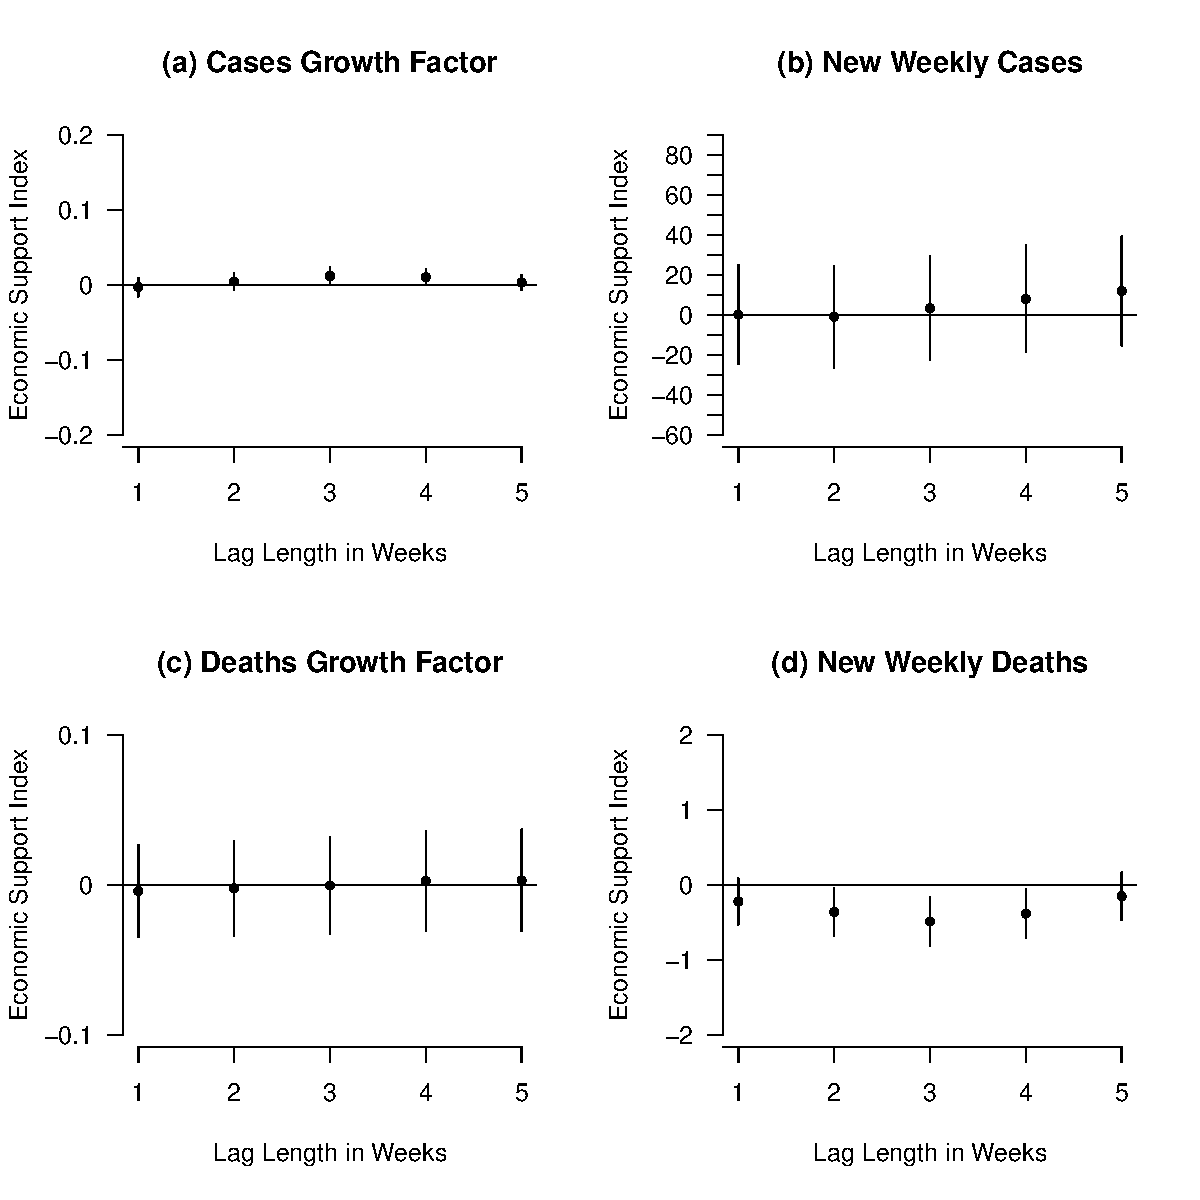
\includegraphics[width=0.8\textwidth]{aesi.pdf}
		\caption{Economic Support Index Coefficients across Four COVID-19 Outcomes, Lagged 1–5 Weeks (Over-Responders)}
		\label{fig:aesi}
	\end{figure}

	\vspace{.25cm}
	
	\noindent The authors also highlight the results from the GRI models in the paper, provided alongside the updated models in Figure 6 below. Note the differences in \texttt{Cases Growth Factor} and \texttt{Deaths Growth Factor} - the Over-Responders  model shows magnitudes-smaller intervals for each, while indicating Government Response has a 2-week lagged effect on cases growth. Additionally, the new models show no statistical significance to the relationship between overall Government Response and \texttt{New Weekly Deaths}.
	
	\begin{figure}[p]
		\centering
		\begin{subfigure}[t]{0.6\textwidth}
			\centering
			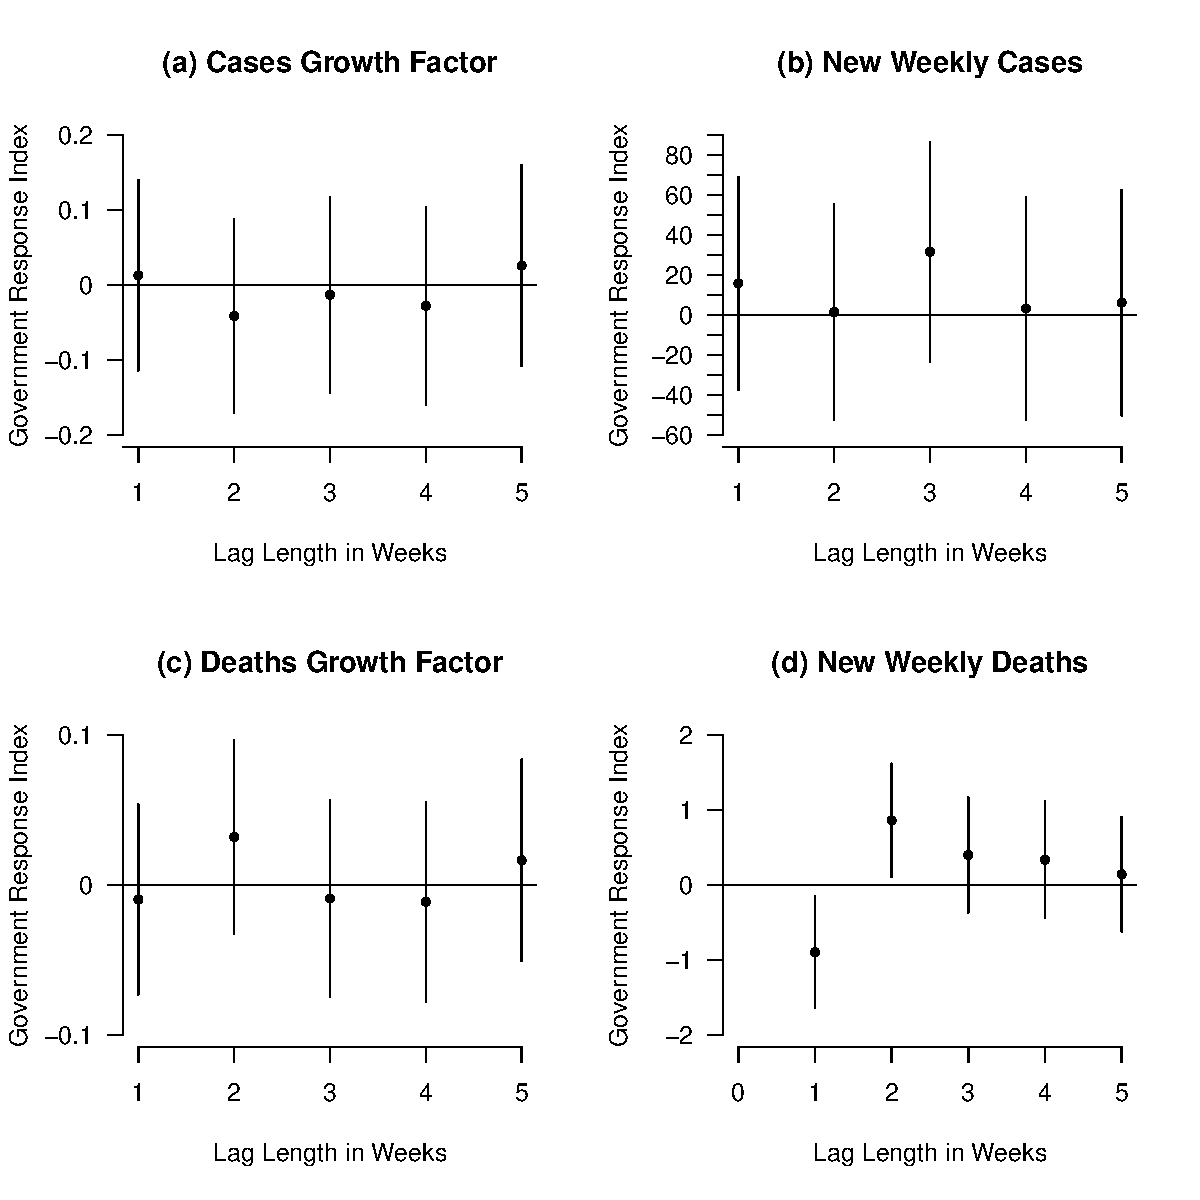
\includegraphics[width=\textwidth]{gri.pdf}
			\caption{Original}
			\label{fig:gri}
		\end{subfigure}
		\vspace{0.5cm} % Add some vertical space between rows
		\begin{subfigure}[b]{0.48\textwidth}
			\centering
			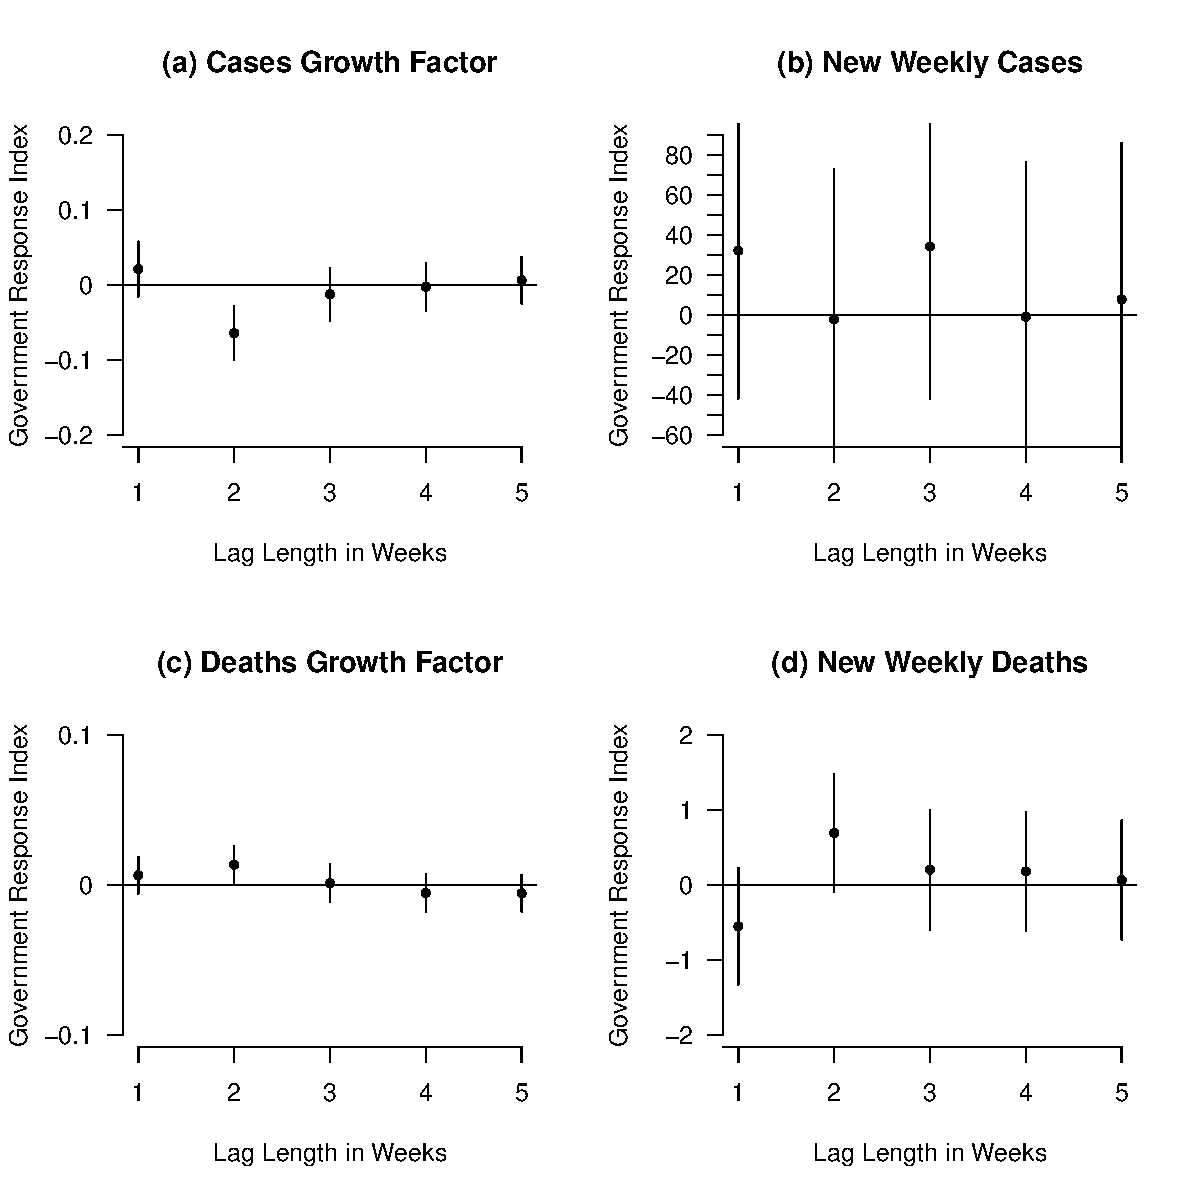
\includegraphics[width=\textwidth]{agri.pdf}
			\caption{Over-Responders}
			\label{fig:agri}
		\end{subfigure}
		\begin{subfigure}[b]{0.48\textwidth}
			\centering
			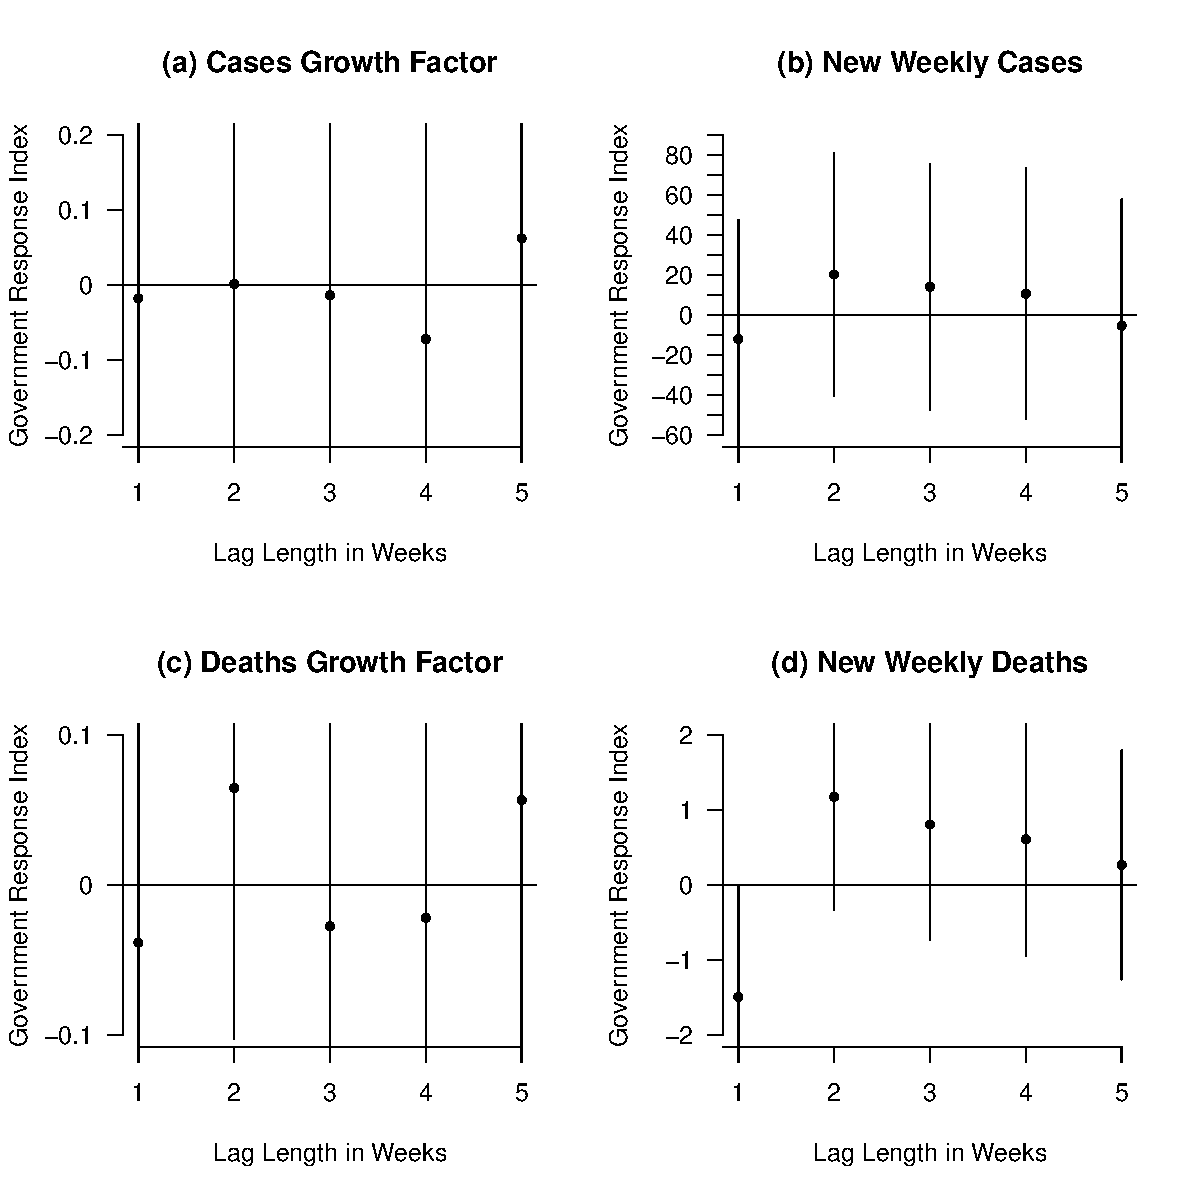
\includegraphics[width=\textwidth]{bgri.pdf}
			\caption{Under-Responders}
			\label{fig:bgri}
		\end{subfigure}
		\caption{Government Response Index Coefficients across Four COVID-19 Outcomes, Lagged 1–5 Weeks}
		\label{fig:all_gri}
	\end{figure}

	\vspace{.25cm}
	
	\noindent Reflecting on the Stringency Index, while the only statistically significant result from the original model indicates an associated reduction in \texttt{New Weekly Deaths} up to the first week, there is no effect among Over-Responders, though over twice the magnitude for Under-Responders (Figure 7). However, the following two lagged weeks indicate an associated increase in \texttt{New Weekly Deaths}. \textbf{This is an important distinction in the dynamics between responses and outcomes for Over- and Under-Responders which is not captured in the original analysis}. Meanwhile, \textbf{over-responses in stringency appear to have an associated decrease by or up to the second week}, though not before or after, which is also not captured in the original analysis.
	
	\begin{figure}[p]
		\centering
		\begin{subfigure}[t]{0.6\textwidth}
			\centering
			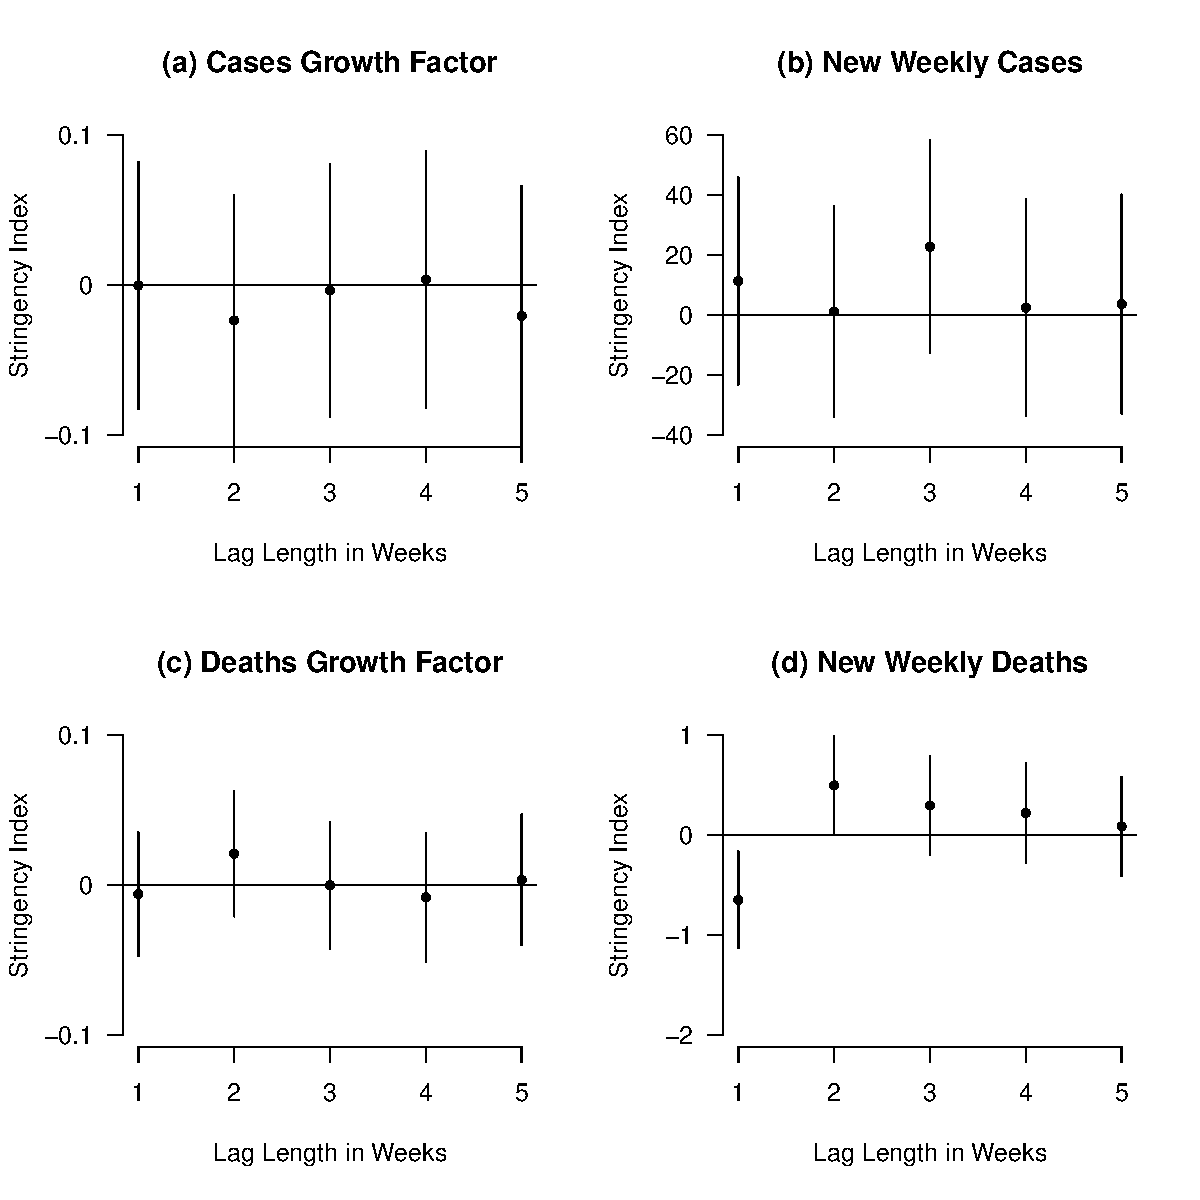
\includegraphics[width=\textwidth]{si.pdf}
			\caption{Original}
			\label{fig:si}
		\end{subfigure}
		\vspace{0.5cm} % Add some vertical space between rows
		\begin{subfigure}[b]{0.48\textwidth}
			\centering
			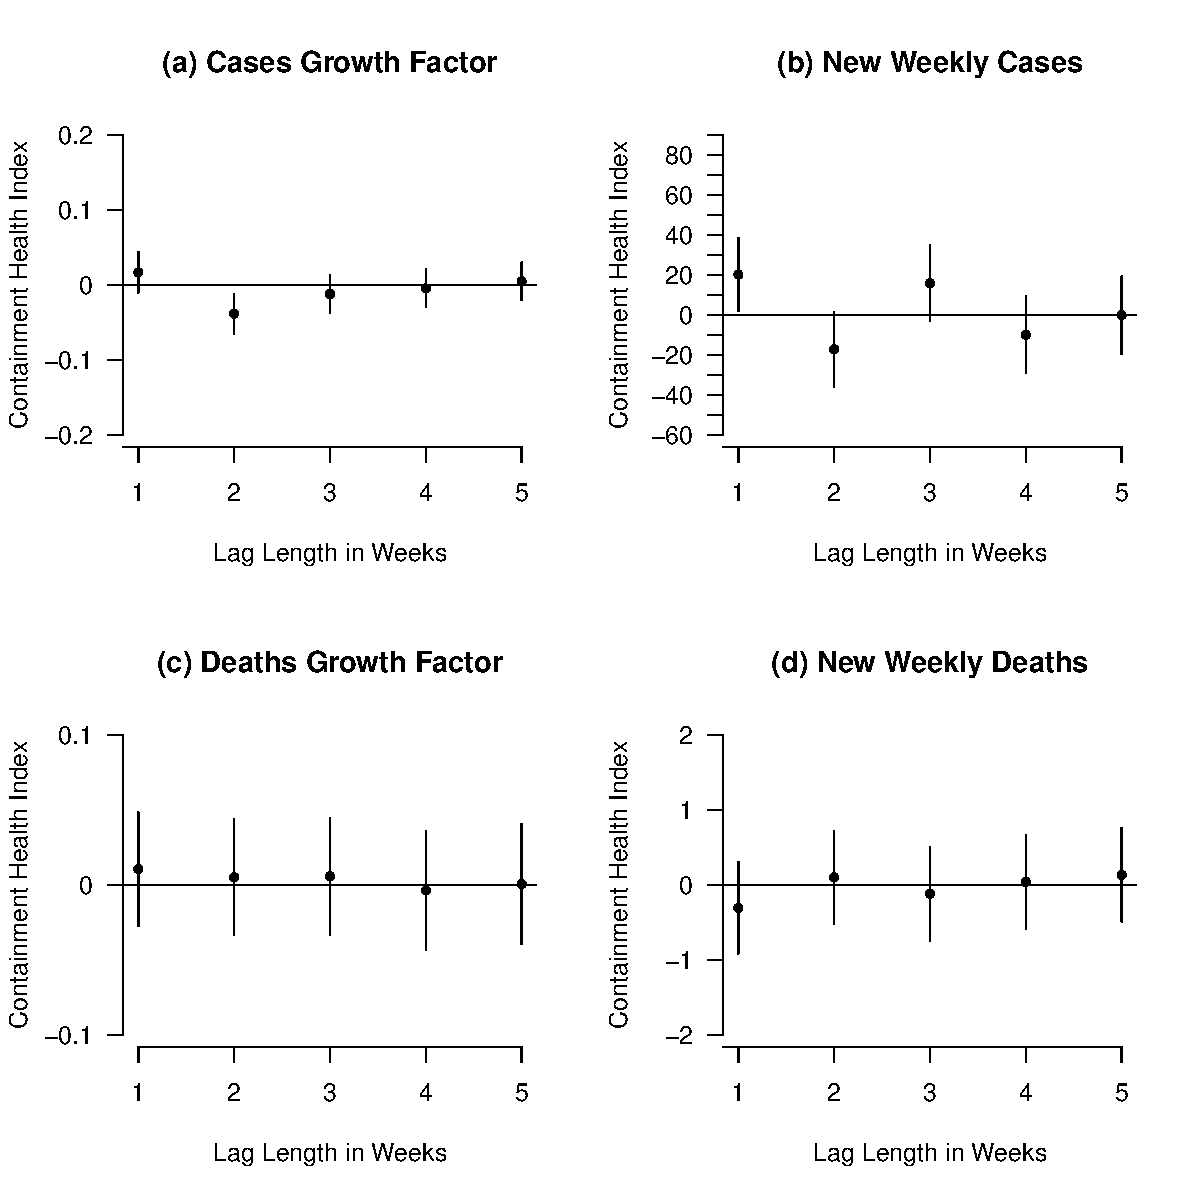
\includegraphics[width=\textwidth]{asi.pdf}
			\caption{Over-Responders}
			\label{fig:asi}
		\end{subfigure}
		\begin{subfigure}[b]{0.48\textwidth}
			\centering
			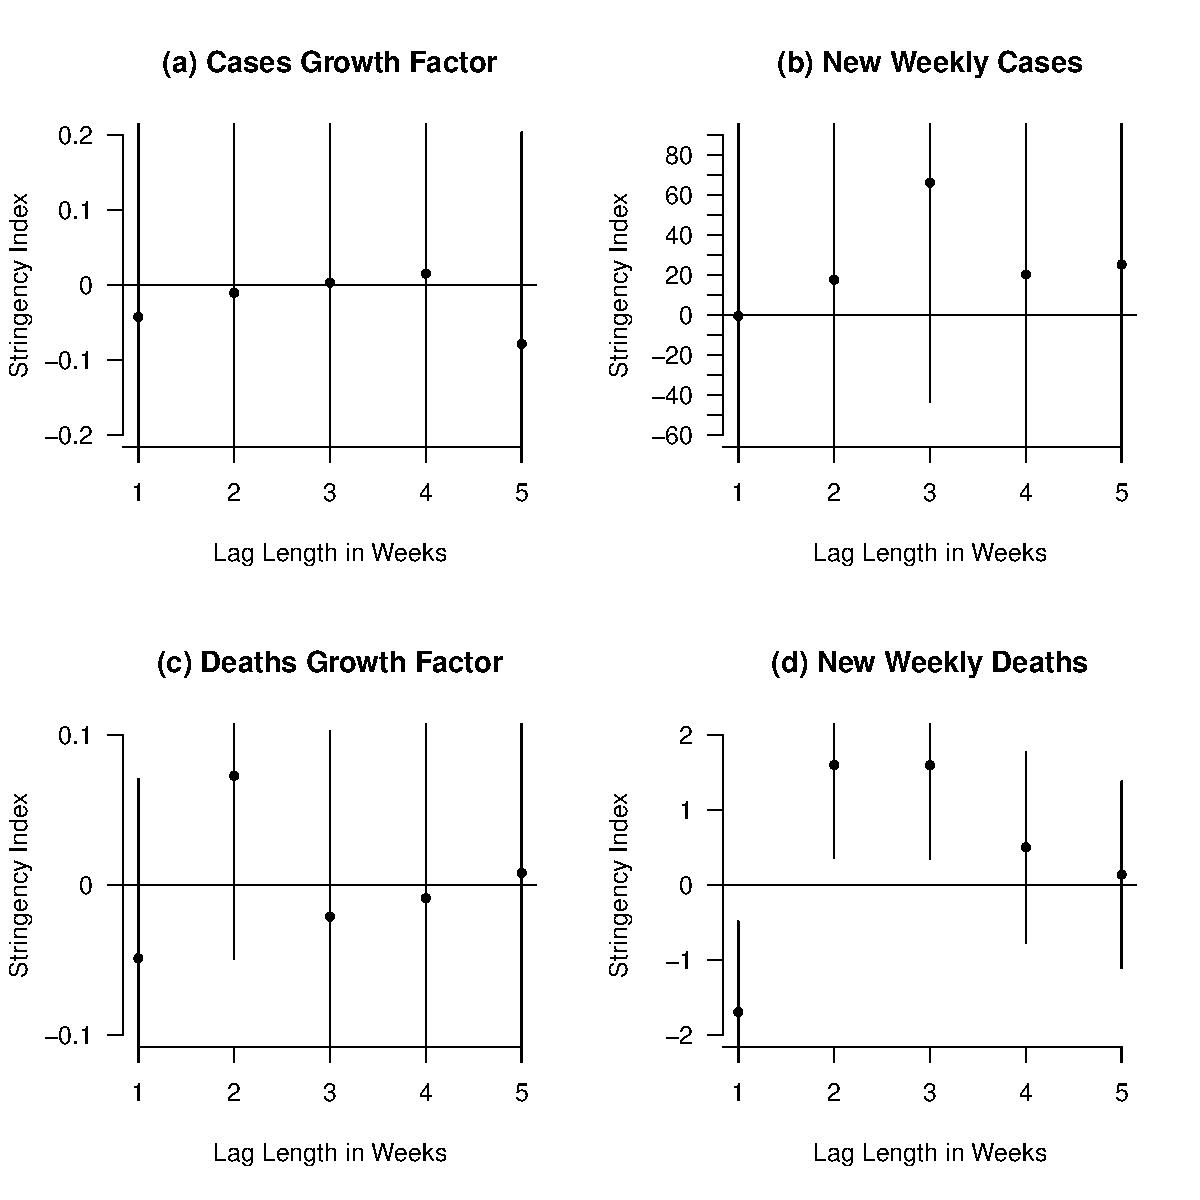
\includegraphics[width=\textwidth]{bsi.pdf}
			\caption{Under-Responders}
			\label{fig:bsi}
		\end{subfigure}
		\caption{Stringency Index Coefficients across Four COVID-19 Outcomes, Lagged 1–5 Weeks}
		\label{fig:all_si}
	\end{figure}
	
	\vspace{.25cm}
	\noindent Lastly, the updated \texttt{Containment Health Index} models (Figure 8) show similar results as for the \texttt{Stringency Index}, the magnitude of the decrease in \texttt{New Weekly Deaths} up to the first week is greater from under-responses and is absent for over-responses, while over-responses have an indicated lagged effect up to and by the second week. The first point refines the original paper's findings, and the second uncovers a dynamic which the original paper did not find.
	
	\begin{figure}[p]
		\centering
		\begin{subfigure}[t]{0.6\textwidth}
			\centering
			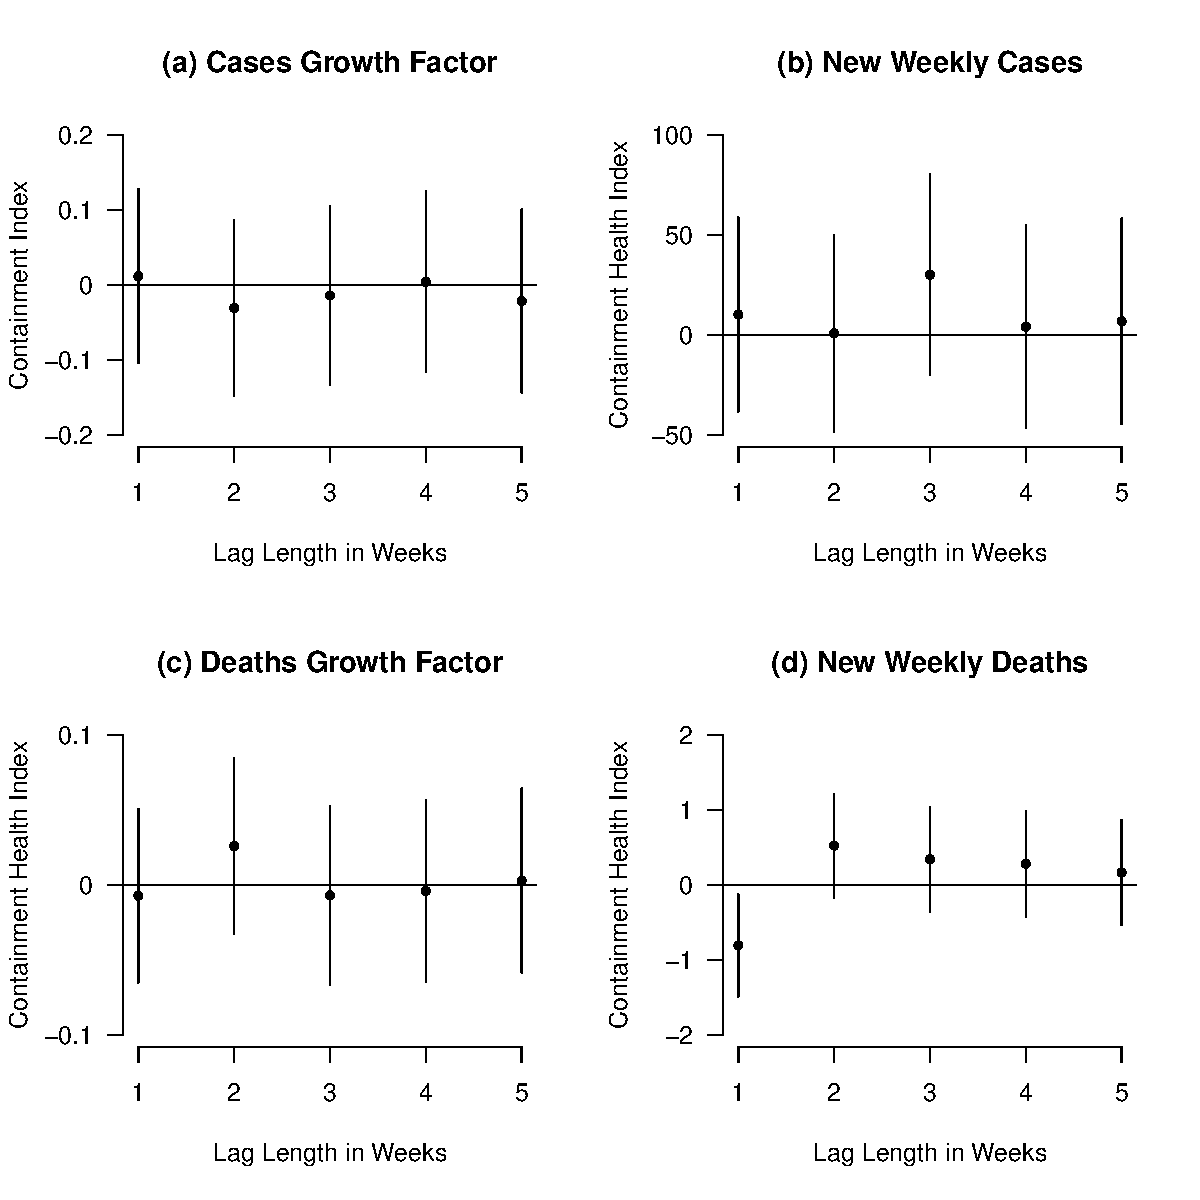
\includegraphics[width=\textwidth]{chi.pdf}
			\caption{Original}
			\label{fig:chi}
		\end{subfigure}
		\vspace{0.5cm} % Add some vertical space between rows
		\begin{subfigure}[b]{0.48\textwidth}
			\centering
			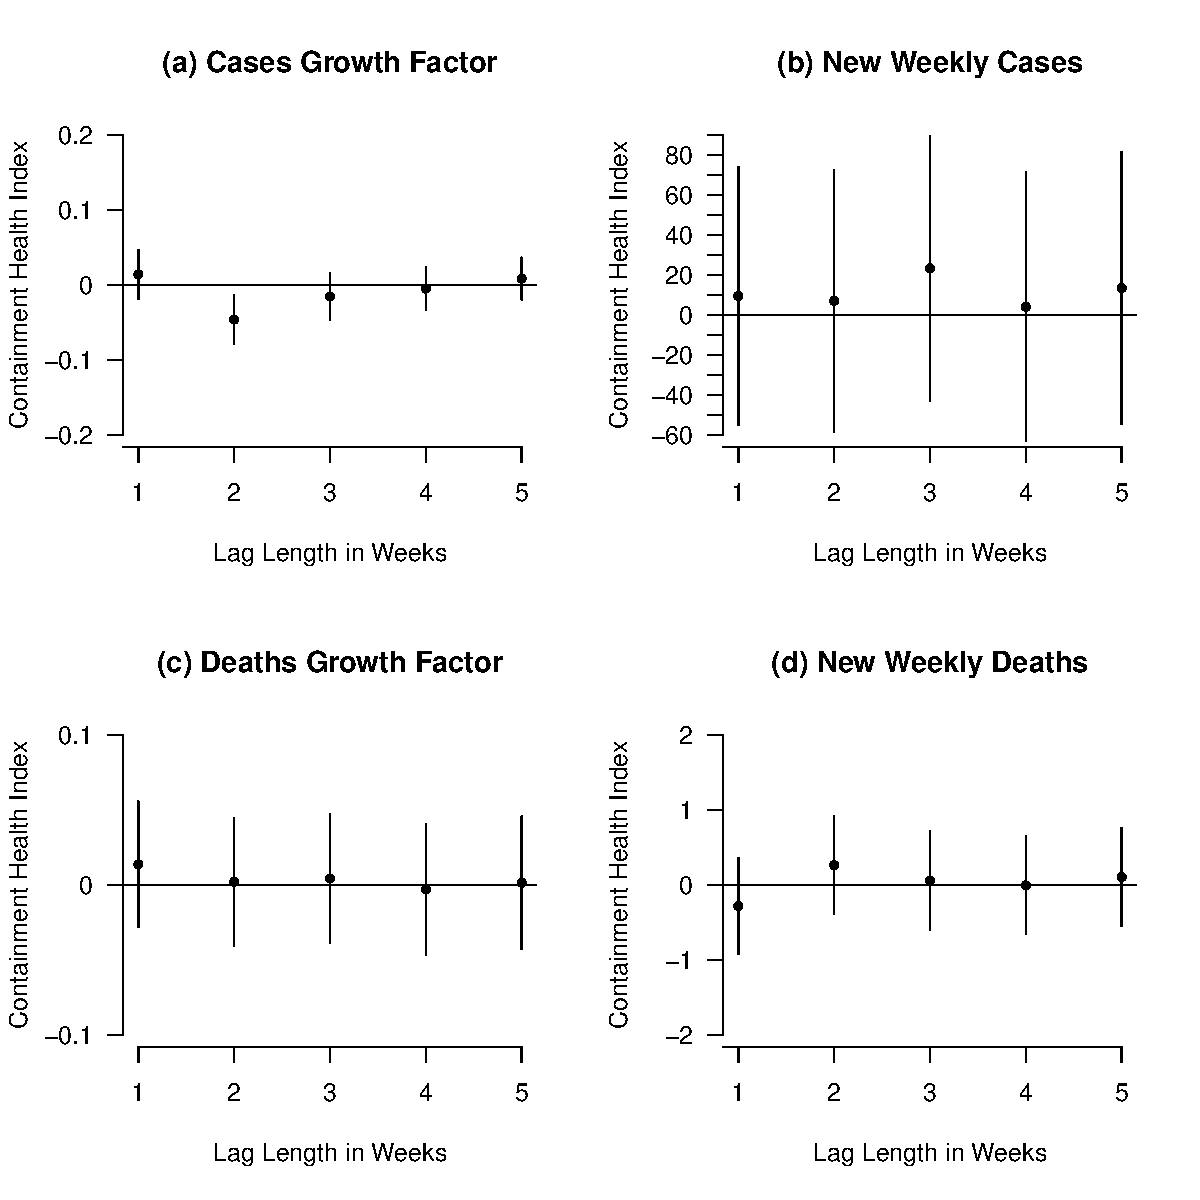
\includegraphics[width=\textwidth]{achi.pdf}
			\caption{Over-Responders}
			\label{fig:achi}
		\end{subfigure}
		\begin{subfigure}[b]{0.48\textwidth}
			\centering
			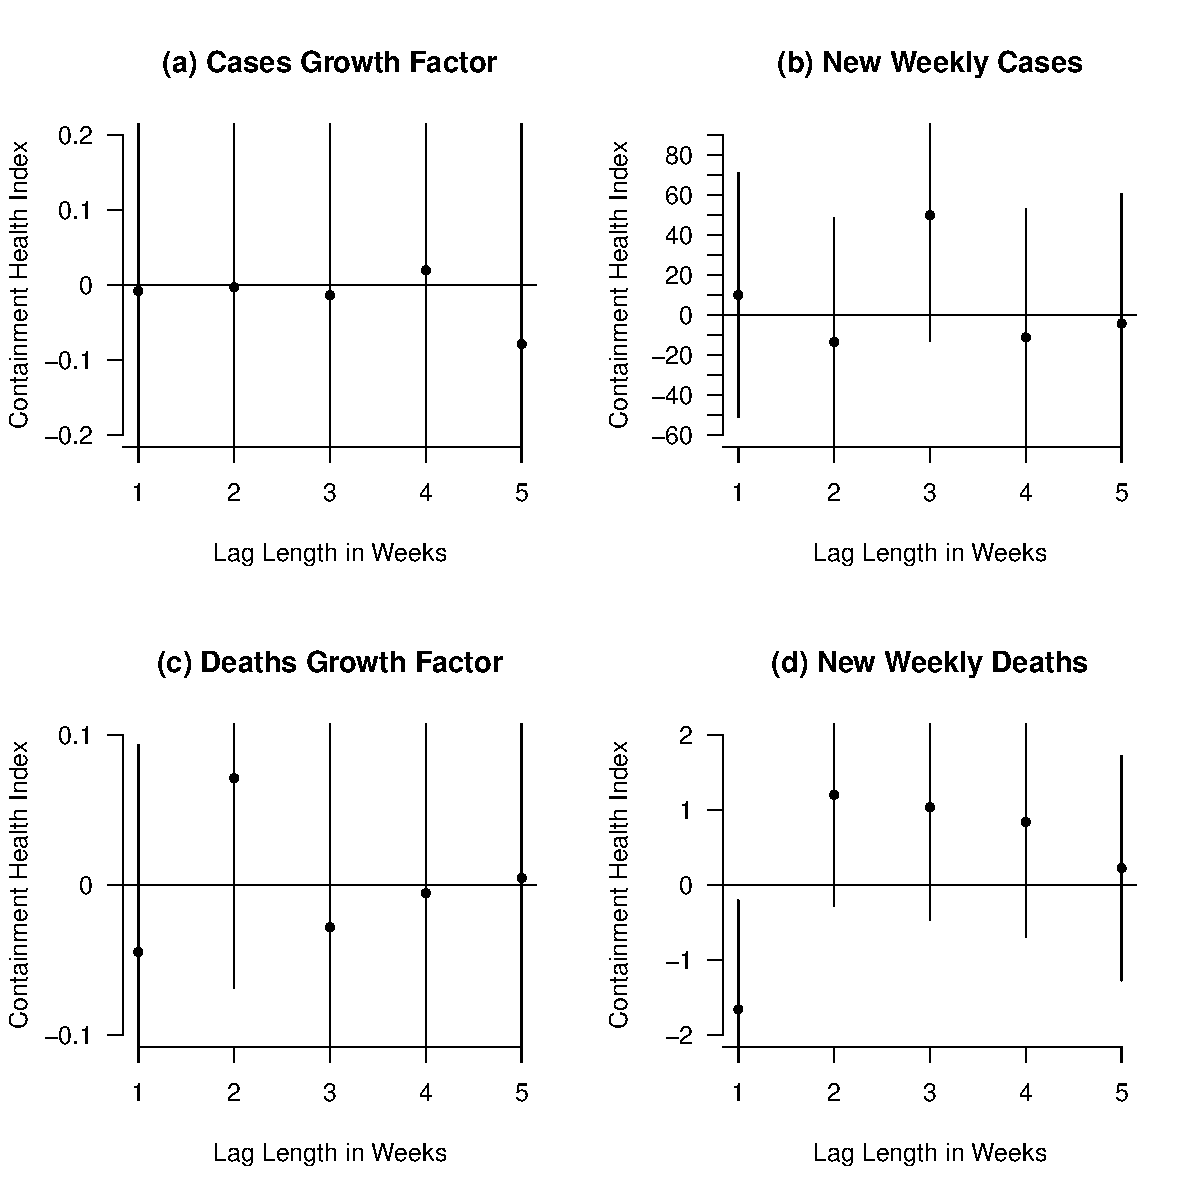
\includegraphics[width=\textwidth]{bchi.pdf}
			\caption{Under-Responders}
			\label{fig:bchi}
		\end{subfigure}
		\caption{Containment Health Index Coefficients across Four COVID-19 Outcomes, Lagged 1–5 Weeks}
		\label{fig:all_chi}
	\end{figure}

	\section*{Findings and Conclusions}
	\vspace{.25cm}	
	
	\noindent The analyses indicate that, for specific outcomes, the dynamics between particular policy responses and COVID-19 outcomes are conditional upon whether a country Over- or Under-Responded. Further, these results provide evidence supporting the effectiveness of some policy responses which was not found by the original analysis. This therefore indicates further work should be done to parse conditional dynamic effects of policy responses and how these relate to dimensions both included and excluded by the analyses used in the original paper and this replication project - from improving the classification method used in this paper, to including socio-political dimensions and other more localised contextual information.

	\vspace{.25cm}	
	
	\noindent My twist has added value and insight to the original paper, however it takes for granted problematic assumptions about the methodology used - namely, the validity of fixed-effects models employed in the original research. Their use in this case remains questionable, even based on the Hausman Tests provided within the replication code provided by the authors. Therefore, further investigation into the appropriate use of linear regression models and in comparative policy analysis work is necessary, as well the issue of inconsistency in the replication and/or interpretation of hypothesis test results.
\end{document}
